\documentclass{amsart}
\usepackage[utf8]{inputenc}

\title{Lab 2}
\author{Allen Williams}
\date{February 19$^{th}$, 2018}

\usepackage{booktabs}
\usepackage{dcolumn}
\usepackage{amsthm}
\usepackage{amsmath}
\usepackage{amssymb}
\usepackage{scrextend}
\usepackage{graphicx}
\usepackage{float}
\usepackage{enumitem}
\usepackage{refstyle}
\usepackage{adjustbox}
\newtheorem*{Theorem}{Theorem}
\newtheorem*{Axiom}{Axiom}
\newtheorem{Problem}{Problem}
\renewcommand\qedsymbol{QED}


\makeatletter
\newcommand{\thickhline}{%
    \noalign {\ifnum 0=`}\fi \hrule height 1pt
    \futurelet \reserved@a \@xhline
}
\newcolumntype{"}{@{\hskip\tabcolsep\vrule width 1pt\hskip\tabcolsep}}
\makeatother


\binoppenalty=\maxdimen
\relpenalty=\maxdimen

\begin{document}

\maketitle

\section*{Objective}
  The objective of this lab exercise was to examine the operation of the Zener diode and to experimentally discover and plot the characteristic curve.
\section*{Procedure}

\begin{enumerate}
\item The circuit in \figref{basic} was constructed with a reverse biased Zener diode in series with a $2.2k\Omega$ resistor.  
\item A voltage varying from 0V to 20V was applied across the circuit with the voltage across the diode and current through the diode recorded in table~\ref{tab:b}.
\item The circuit of \figref{practical} was analyzed theoretically with $V=2V$, $V=5V$, $V=10V$, $V=15V$, and $V=20V$ using $R_1=2.2k\Omega$ and $R_2=4.7k\Omega$.  The voltage across the diode and current through the diode were recorded in table \ref{tab:p}.
\item The circuit of \figref{practical} was constructed and the voltage across the diode and current through the diode were measured and recorded in table \ref{tab:p} and compared with the theoretical values calculated in step 3.
\end{enumerate}

\section*{Discussion}
The first section of the experiment was the analysis of the circuit in \figref{basic} which consisted of a reverse biased Zener diode in series with a resistor and a voltage source.  A $2.2k\Omega$ resistor was used and voltages of $0V$, $1V$, $2V$, $5V$, $10V$, $15V$, and $20V$ were applied across the circuit.  The Zener diode used had a rated $V_Z$ of $4.7V$.  The voltage across the diode and current through the diode were recorded at each of the input voltages with the results summarized in table~\ref{tab:b} in the appendix. \figref{G1} is a graph of the data in table \ref{tab:b} showing the relationship between the voltage across the reverse biased Zener diode and the current passing through the reverse biased Zener diode.
\begin{figure}[H]
\caption{Reverse Biased Zener Diode}
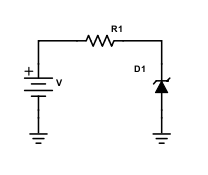
\includegraphics[width=\textwidth]{L2F1.png}
\label{fig:basic}
\end{figure}
The diode behaved as expected based on theory.  For voltages lower than the rated $V_Z$ for the diode the effective resistance of the diode was infinite and all of the circuit voltage dropped across the diode.  As the voltage approached $V_Z$ the diode began to have lower resistance and allow some current to flow.  Although a small current began to flow with as little as $3.700V$ across the diode, the current became much more noticeable as the voltage measured across the diode approached the rated $V_Z$, $4.7V$.  The voltage across the diode seemed to approach a limit of $V_Z=4.7V$ as the voltage applied to the circuit was increased, meaning as the voltage applied to the entire circuit was increased the proportion of that change in voltage that dropped across the Zener diode became progressively smaller while the proportion of the change in voltage that dropped across the resistor became progressively larger.

The instantaneous resistance, which was calculated as $r_{diode}=\frac{\Delta V_{diode}}{\Delta I_{diode}}$ was minimized among the values in table~\ref{tab:b} using the data in the last two rows, so $r_{diode}=\frac{4.602V-4.492V}{0.007A-0.0048A}=50\Omega$.

The second portion of this experiment involved the practical analysis of a circuit containing a reverse biased Zener diode.  For this portion of the experiment the circuit of \figref{practical} was used.  The voltage across the diode and current through the diode were first calculated using theory.  Because the diode is connected in parallel with $R_2$, the voltage across the diode must be the same as the voltage across $R_2$.  By assuming the diode was inactive and calculating the voltage drop across $R_2$ in the resulting series circuit using voltage division, the voltage across $R_2$, and therefore also the voltage across the diode, was determined to be less than $V_Z$ when the circuit voltage was either $2V$ or $5V$, since $2V\cdot \frac{4.7k\Omega}{4.7k\Omega+2.2k\Omega}=1.362V$, and $5V\cdot \frac{4.7k\Omega}{4.7k\Omega+2.2k\Omega}=3.406V$ hence, the diode was determined to be inactive when $2V$ or $5V$ were applied to the circuit.  In these cases the theoretical voltage across the diode was equal to the theoretical voltage across $R_2$ in a circuit with an open replacing the diode and the theoretical current through the diode was $0mA$.  

For the applied voltages of $10V$ or more the voltage across $R_2$ with the Zener considered inactive are greater than the Zener potential $V_Z$, so the Zener was considered active and the voltage across $R_2$ was limited to $V_Z=4.7V$.  The voltage across $R_1$ could then be computed as $V_{R_1}=V_{SRC}-4.7V$ by Kirchoff's Voltage Law.  The current through $R_1$ could then be computed by $I_{R_1}=\frac{V_{R_1}}{R_1}$.  The current through the diode could then be computed by $I_D=I_{R_1}-\frac{V_{R_2}}{R_2}$ and since $V_{R_2}$ was assumed to be $4.7V$, $I_D=I_{R_1}-\frac{4.7V}{4.7k\Omega}=I_{R_1}-1mA$. As an example, when the applied voltage was $15V$, the Zener was considered active so $4.7V$ dropped across $R_2$.  By Kirchoff's Voltage Law, this meant $15V-4.7V=10.3V$ must have dropped across $R_1$, so $I_{R_1}=\frac{10.3V}{2.2k\Omega}=4.68mA$.  By Kirchoff's Current Law the current through the diode must equal the current through $R_1$ minus the current through $R_2$, so $I_D=4.68mA-\frac{4.7V}{4.7k\Omega}=4.68mA-1.00mA=3.68mA$.  The results of this analysis are summarized in columns two and three of table~\ref{tab:p} in the appendix.

\begin{figure}[H]
\caption{Practical Analysis with Zener Diode}
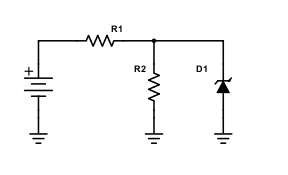
\includegraphics[width=\textwidth]{L2F2.png}
\label{fig:practical}
\end{figure}

The circuit of \figref{practical} was then constructed and 
the voltage across the diode and the current through the diode were measured and compared to the theoretical values.  As long as the voltage across the diode was well below or very close to $V_Z=4.7V$, the diode was very well behaved compared to its theoretical values. Although the model of a diode turning on at $V_Z$ and beginning to conduct is a useful approximation, it actually began to allow small amounts of current through at voltages lower than $V_Z$, even as low as $3.1V$.  Because of this the assumption that the voltage across the Zener was always equal to $V_Z$ led to percent errors as large as $21\%$ when the voltage across the Zener was just below $V_Z$.  As the applied voltage in the circuit was increased the voltage across the Zener approached $V_Z$ and the percent errors decreased.  

\section*{Conclusion}
This lab experiment illustrated the uses and characteristics of the Zener diode.  The approximation that the voltage across a Zener diode is always equal to $V_Z$, at least when enough voltage is applied to the circuit, was found to be valid in a wide range of voltages, but led to significant errors for a small range of applied voltages.  


\section*{Appendix}

\begin{table}[H]
    \centering
    \caption{V and I for the circuit in \figref{basic}}
    \begin{tabular}{|c"c|c|} \hline
        $V(Volts)$ & $V_D(Volts)$ & $I_D(milliAmps)$ \\ \thickhline
        0 & 0.00210 & 0 \\\hline
        1 & 0.981 & 0 \\\hline
        2 & 1.973 & 0 \\\hline
        5 & 3.700 & 0.6 \\\hline
        10 & 4.289 & 2.6 \\\hline
        15 & 4.492 & 4.8 \\\hline
        20 & 4.602 & 7.0 \\\hline
    \end{tabular}
    \label{tab:b}
\end{table}

\begin{figure}[H]
    \centering
    \caption{Reverse Biased Zener Diode Current v. Voltage}
    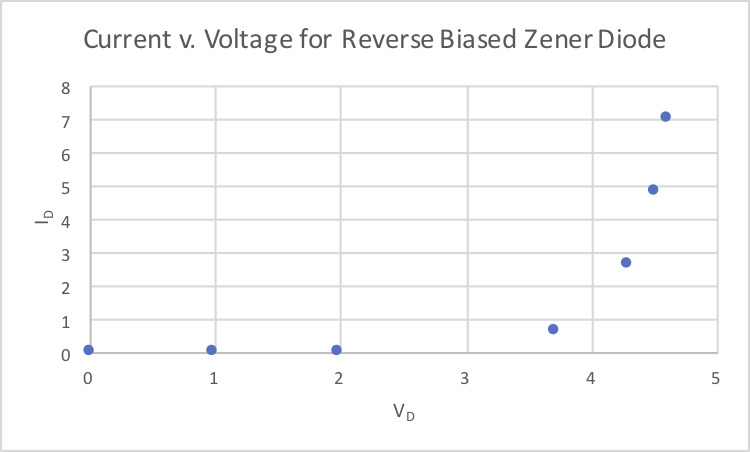
\includegraphics[width=\textwidth]{L2G1.png}
    \label{fig:G1}
\end{figure}

\begin{table}[H]
    \centering
    \caption{Theoretical and Measured Voltage and Current for the Circuit in \Figref{practical}}
    \resizebox*{\textwidth}{!}{
    \begin{tabular}{|c"c|c|c|c|c|c|} \hline
        $V(Volts)$ & $V_{D\text{ }Theory}(Volts)$ & $I_{D\text{ }Theory}(milliAmps)$ & $V_{D\text{ }Exp}(Volts)$ & $I_{D\text{ }Exp}(milliAmps)$ & $\%Dev\text{ }V_D(\%)$ & $\%Dev\text{ }I_D(\%)$ \\\thickhline
        2 & 1.362 & 0 & 1.337 & 0 & 1.836 & n/a \\\hline
        5 & 3.406 & 0 & 3.153 & 0.2 & 7.428 & n/a \\\hline
        10 & 4.700 & 1.410 & 4.143 & 1.800 & 11.85 & 21.67 \\\hline
        15 & 4.700 & 3.680 & 4.425 & 3.800 & 5.851 & 3.158 \\\hline
        20 & 4.700 & 5.950 & 4.563 & 6.000 & 2.915 & 0.8333 \\\hline
    \end{tabular}}
    \label{tab:p}
\end{table}

\end{document}
